\begin{figure}[H]
\captionsetup{width=.75\textwidth}
    \centering
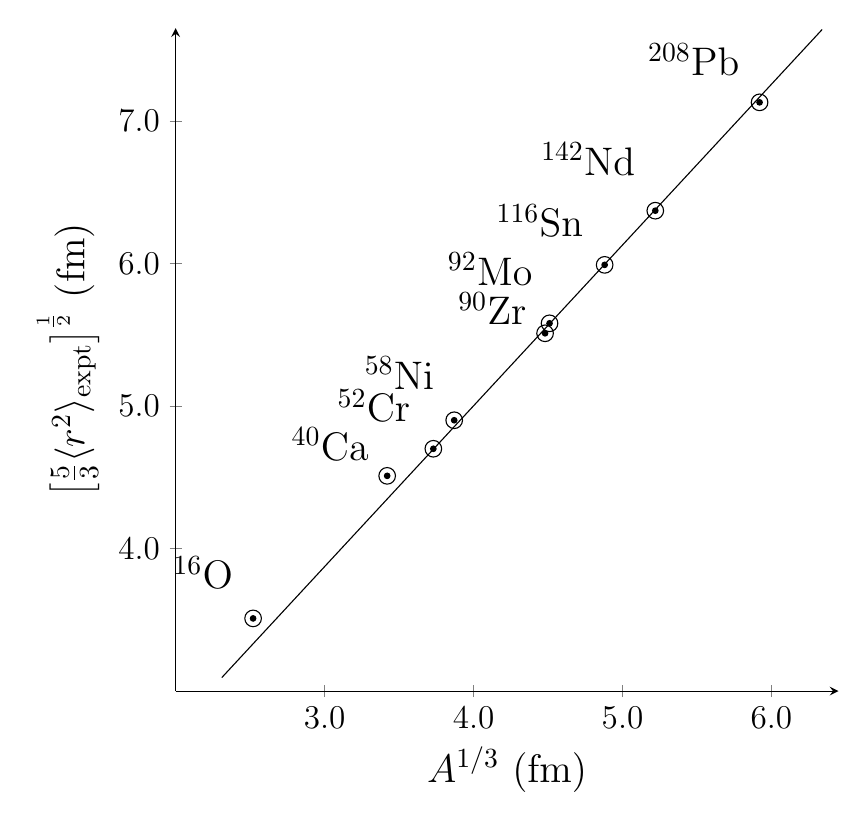
\begin{tikzpicture}
\begin{axis}[
    width=10cm, height=10cm,
    axis lines=left,
    xmin=2, xmax=6.45,
    ymin=3, ymax=7.65,
    xtick={3.0,4.0,5.0,6.0},
    ytick={4.0,5.0,6.0,7.0},
    yticklabel style={/pgf/number format/fixed, /pgf/number format/fixed zerofill, /pgf/number format/precision=1},
    xticklabel style={/pgf/number format/fixed, /pgf/number format/fixed zerofill, /pgf/number format/precision=1},
    xlabel={$A^{1/3}$ (fm)},
    ylabel={$\left[\frac{5}{3}\langle r^2\rangle_{\mathrm{expt}}\right]^{\frac{1}{2}}$ (fm)},
    xlabel style={font=\Large},
    ylabel style={font=\Large},
    tick label style={font=\large},
    clip=false,
]

% Straight-line guide
\addplot[black, thin, domain=2.31:6.34] {1.128*(x-2.31)+3.095};

% Data points (circled dots)
\addplot[only marks, mark=*, mark size=1pt] coordinates {
    (2.52,3.51) (3.42,4.51) (3.73,4.70) (3.87,4.90)
    (4.48,5.51) (4.51,5.58) (4.88,5.99) (5.22,6.37) (5.92,7.13)
};
\addplot[only marks, mark=o, mark size=3pt] coordinates {
    (2.52,3.51) (3.42,4.51) (3.73,4.70) (3.87,4.90)
    (4.48,5.51) (4.51,5.58) (4.88,5.99) (5.22,6.37) (5.92,7.13)
};

% Nuclide labels
\node[anchor=south east, font=\Large] at (axis cs:2.45,3.65) {$^{16}$O};
\node[anchor=south east, font=\Large] at (axis cs:3.36,4.55) {$^{40}$Ca};
\node[anchor=south east, font=\Large] at (axis cs:3.64,4.82) {$^{52}$Cr};
\node[anchor=south east, font=\Large] at (axis cs:3.80,5.05) {$^{58}$Ni};
\node[anchor=south east, font=\Large] at (axis cs:4.42,5.50) {$^{90}$Zr};
\node[anchor=south east, font=\Large] at (axis cs:4.46,5.78) {$^{92}$Mo};
\node[anchor=south east, font=\Large] at (axis cs:4.80,6.12) {$^{116}$Sn};
\node[anchor=south east, font=\Large] at (axis cs:5.15,6.55) {$^{142}$Nd};
\node[anchor=south east, font=\Large] at (axis cs:5.85,7.25) {$^{208}$Pb};

\end{axis}
\end{tikzpicture}
    \caption{Nuclear rms charge radii compared to the liquid drop model. 
    Almost exact for \(A\geq90\), deviation for \(A < 90\) due to surface 
    diffuseness. Adapted from fig. 1.7 in \textit{Primer} \anth}
    \label{rms_vs_A}
\end{figure}

